\section{Log-gamma moments: from a classical expansion to a sharp error law}
\label{sec:moments}

For \(n\geq 0\), write
\[
 M_n=\int_0^1\log^n\Gamma(x)\dd x,\qquad m_n=\frac{M_n}{n!}.
\]
The convention \(M_0=1\) is understood. The classical expansion of
Amdeberhan et al.~\cite{ACEMKM} is
\begin{equation}\label{eq:classical-moment}
 m_n\sim\sum_{k\geq1}\frac{(-1)^{k-1}b_k}{k^n},\qquad
 b_k=\frac1k[z^{k-1}]\Gamma(1-z)^k>0.
\end{equation}
Here and below an infinite asymptotic expansion means that its truncation
index is fixed before \(n\to\infty\). It does not assert convergence of the
infinite sum for any fixed \(n\). Our aim is to determine the growth of
\(b_k\), locate the least term, and prove the error when the truncation
index grows with \(n\).

\subsection{Inverse coordinates and residues}

Let \(g\) denote the inverse germ at zero of the entire reciprocal gamma
function:
\[
 \frac1{\Gamma(g(t))}=t,\qquad g(0)=0,\qquad g'(0)=1.
\]
For \(0\leq t\leq1\), use the real continuation with \(0\leq g(t)\leq1\).
It exists uniquely: \(\psi(x)<0\) for \(0<x\leq1\), because
\(\psi\) is increasing and \(\psi(1)=-\gamma<0\).
Thus \(1/\Gamma(x)\) is strictly increasing from 0 to 1 on this interval.
The inverse under discussion is not the increasing large-argument inverse
of \(\Gamma\).

\begin{proposition}[Inverse and Mellin descriptions]\label{prop:inverse}
With \(c_k=(-1)^{k-1}b_k\), the inverse germ satisfies
\begin{equation}\label{eq:g-series}
 g(t)=\sum_{k\geq1}c_kt^k,\qquad
 B(t):=-g(-t)=\sum_{k\geq1}b_kt^k=t\Gamma(1-B(t)).
\end{equation}
For \(n\geq1\),
\begin{equation}\label{eq:layercake}
 m_n=\frac1{(n-1)!}\int_0^\infty y^{n-1}g(e^{-y})\dd y.
\end{equation}
The function
\[
 \mathcal M(s)=\int_0^1\Gamma(x)^s\dd x,\qquad \Re s<1,
\]
continues meromorphically to \(\C\), has only simple poles at the
positive integers, and
\begin{equation}\label{eq:mgf-res}
 \Res_{s=k}\mathcal M(s)=-k c_k,\qquad
 [s^n]\mathcal M(s)=m_n.
\end{equation}
Every positive integer is an actual pole.
\end{proposition}

\begin{proof}
The inverse equation is \(g=t\Gamma(1+g)\). Lagrange inversion gives
\([t^k]g=k^{-1}[z^{k-1}]\Gamma(1+z)^k=c_k\).
The expansion
\begin{equation}\label{eq:phi}
 \Phi(z):=\Gamma(1-z)
 =\exp\left(\gamma z+\sum_{j\geq2}\frac{\zeta(j)}jz^j\right)
\end{equation}
has strictly positive coefficients. This proves the positivity in
\eqref{eq:classical-moment} and the equation for \(B\).
The function \(x\mapsto\log\Gamma(x)\) decreases from infinity to zero;
the measure of the set where it exceeds \(y\) is \(g(e^{-y})\).
The layer-cake formula for a nonnegative function gives
\eqref{eq:layercake}.

For the last assertion, set \(H(x,s)=\Gamma(1+x)^s\), using its analytic
logarithm for \(|x|<1\). Write
\(H(x,s)=\sum_{j\geq0}a_j(s)x^j\), with each \(a_j\) entire in \(s\).
Choose \(0<d<1\), split the integral at \(d\), and subtract a finite
Taylor polynomial on \([0,d]\). For every integer \(J\geq0\),
\begin{align}
 \mathcal M(s)
 &=\sum_{j=0}^J\frac{a_j(s)d^{j+1-s}}{j+1-s}
   +\int_0^d x^{-s}\left(H(x,s)-\sum_{j=0}^Ja_j(s)x^j\right)\dd x
   +\int_d^1\Gamma(x)^s\dd x. \label{eq:meromorphic}
\end{align}
The remainder integral is holomorphic in \(\Re s<J+2\), locally
uniformly there. Taking \(J\) arbitrarily large proves continuation.
At \(s=k\), the residue is \(-a_{k-1}(k)=-k c_k\), which is nonzero.
Differentiation under the original integral near \(s=0\) proves the
coefficient identity.
\end{proof}

Subtracting the first \(K\) polar parts \(k c_k/(k-s)\) from
\(\mathcal M\) leaves a function holomorphic in \(|s|<K+1\).
Cauchy's estimate, after subtracting one extra pole, consequently gives
the rigorous fixed-length version
\begin{equation}\label{eq:fixed-remainder}
 m_n=\sum_{k=1}^K\frac{c_k}{k^n}
       +\frac{c_{K+1}}{(K+1)^n}
       +O_{K,R}(R^{-n}),\qquad K+1<R<K+2.
\end{equation}
This recovers the classical expansion by a meromorphic argument; it is
not presented as a new asymptotic scale.

For exact coefficient generation, define \(a_0(s)=1\) and
\[
 a_j(s)=\frac{s}{j}\sum_{\ell=1}^j q_\ell a_{j-\ell}(s),\qquad
 q_1=\gamma,\quad q_\ell=\zeta(\ell)\quad(\ell\geq2).
\]
Then \(b_k=a_{k-1}(k)/k\). This recurrence involves only rational
arithmetic in the formal symbols \(\gamma,\zeta(2),\ldots\).
For example,
\begin{align*}
 b_1&=1,& b_2&=\gamma,&
 b_3&=\frac{3\gamma^2+\zeta(2)}2,\\
 b_4&=\frac{8\gamma^3+6\gamma\zeta(2)+\zeta(3)}3,\\
 b_5&=\frac{125\gamma^4}{24}
      +\frac{25\gamma^2\zeta(2)}4+\frac{5\gamma\zeta(3)}3
      +\frac{5\zeta(2)^2}{8}+\frac{\zeta(4)}4.
\end{align*}
These homogeneous polynomials have weight \(k-1\) under the formal
assignments \(\mathrm{wt}(\gamma)=1\) and
\(\mathrm{wt}(\zeta(j))=j\). No independence assumption is needed to
generate or verify them.

\subsection{The singularity that controls late coefficients}

\begin{theorem}[Late coefficients]\label{thm:late}
There is a unique \(\tau\in(0,1)\) satisfying \(\psi(-\tau)=0\).
Define
\begin{equation}\label{eq:constants}
 \rho=\frac{\tau}{\Gamma(1-\tau)},\qquad
 \Lambda=-\log\rho,\qquad
 C=\frac1{\sqrt{2\pi\psi'(-\tau)}}.
\end{equation}
Then \(B\) has radius of convergence \(\rho\), its only singularity on
that circle is \(\rho\), and it has a square-root expansion there.
In particular,
\begin{equation}\label{eq:late}
 b_k=C\rho^{-k}k^{-3/2}
       \left(1+\frac{d_1}{k}+O(k^{-2})\right).
\end{equation}
A complete expansion in powers of \(1/k\) exists. If
\(\kappa_j=((z\,\partial_z)^j\log\Phi(z))|_{z=\tau}\), so that
\(\kappa_1=1\), then
\begin{equation}\label{eq:d1}
 d_1=-\frac1{2\kappa_2}
      +\frac{\kappa_3}{2\kappa_2^2}
      +\frac{\kappa_4}{8\kappa_2^2}
      -\frac{5\kappa_3^2}{24\kappa_2^3}.
\end{equation}
Equivalently, with \(P=\psi'(-\tau)\), \(Q=\psi''(-\tau)\),
and \(R=\psi'''(-\tau)\),
\begin{equation}\label{eq:d1-polygamma}
 d_1=\frac{R}{8P^2}-\frac{5Q^2}{24P^3}.
\end{equation}
\end{theorem}

\begin{proof}
The characteristic equation for \(B=t\Phi(B)\) is
\(\tau\Phi'(\tau)=\Phi(\tau)\).
Since \(\Phi'/\Phi=-\psi(1-z)\), recurrence of the digamma function
turns this into \(\psi(-\tau)=0\).
Alternatively \(z\Phi'(z)/\Phi(z)=\gamma z+\sum_{j\geq2}\zeta(j)z^j\)
is strictly increasing from 0 to infinity on \((0,1)\), proving
existence and uniqueness. The function \(z/\Phi(z)\) increases up to
\(\tau\) and then decreases.

The power series solution has nonnegative coefficients and reaches
\(B(\rho)=\tau\). One elementary justification is to iterate
\(B_{j+1}=t\Phi(B_j)\), starting with \(B_0=0\), for \(0\leq t<\rho\);
monotonicity and the smaller real solution bound the iterates.
Monotone convergence and inversion give the limit at \(\rho\).
At the characteristic point,
\[
 \Phi''(\tau)/\Phi(\tau)
 =\psi'(1-\tau)+\psi(1-\tau)^2
 =\psi'(1-\tau)+\tau^{-2}=\psi'(-\tau)>0.
\]
Local inversion therefore gives
\begin{equation}\label{eq:puiseux}
 B(t)=\tau-\alpha\sqrt{1-t/\rho}+O(1-t/\rho),
 \qquad \alpha=\sqrt{\frac2{\psi'(-\tau)}}.
\end{equation}
There is a convergent Puiseux expansion, with integral and half-integral
powers.

For completeness, there are no other dominant singularities.
Absolute convergence at \(|t|=\rho\) follows from \(B(\rho)=\tau\).
If \(t\neq\rho\) lies on that circle, the positive coefficients of
\(t\) and \(t^2\) give \(|B(t)|<\tau\). Hence
\[
 |t\Phi'(B(t))|\leq\rho\Phi'(|B(t)|)<\rho\Phi'(\tau)=1.
\]
The analytic implicit-function theorem continues \(B\) across every such
point. Compactness, together with local square-root inversion at \(\rho\),
supplies a slit disk \(|t|<\rho+\epsilon\) with the sole cut issuing from
\(\rho\). This is the smooth implicit-function mechanism of
analytic combinatorics~\cite{FS}, with its hypotheses verified here.
Transfer of \((1-t/\rho)^{1/2}\) gives
\(C=\alpha/(2\sqrt\pi)\) and the full expansion.

We also give a direct computation of the first correction.
Lagrange's coefficient integral on \(|z|=\tau\) is
\[
 b_k=\frac{\tau\rho^{-k}}{2\pi k}
 \int_{-\pi}^{\pi}
 \exp\!\left(k\{\log\Phi(\tau e^{i\theta})-\log\Phi(\tau)-i\theta\}\right)
 e^{i\theta}\dd\theta.
\]
Positivity and aperiodicity make the modulus strictly smaller away from
\(\theta=0\). At zero the exponent is
\(-\kappa_2\theta^2/2-i\kappa_3\theta^3/6
 +\kappa_4\theta^4/24+\cdots\).
After \(\theta=u/\sqrt{k}\), Gaussian integration gives respectively
\(-1/(2\kappa_2)\), \(\kappa_3/(2\kappa_2^2)\),
\(\kappa_4/(8\kappa_2^2)\), and
\(-5\kappa_3^2/(24\kappa_2^3)\).
Also \(\kappa_2=\tau^2\psi'(-\tau)\), so the leading constant agrees
with \eqref{eq:constants}. Taylor expansion to any fixed order, with an
exponentially small outer arc, proves the complete saddle expansion.
\end{proof}

Numerical values, used only as orientation, are
\begin{align*}
 \tau&=0.5040830082644554092582693045333024989\ldots,\\
 \rho&=0.2821158090062980421537966006204637282\ldots,\\
 \Lambda&=1.2654376221108656133820359111654739922\ldots,\\
 C&=0.1334277613094452848960205705394178243\ldots,\\
 d_1&=0.3019628287812052411245866827164781138\ldots.
\end{align*}

\begin{corollary}[Divergence and least terms]\label{cor:least}
For every fixed \(n\), the terms of the infinite series in
\eqref{eq:classical-moment} eventually grow in magnitude and do not tend
to zero. Its smallest terms occur at
\[
 k=\frac{n+3/2}{\Lambda}+O(1).
\]
For any integer \(N\) with \(N\Lambda-n\) bounded,
\begin{equation}\label{eq:least-size}
 \frac{b_N}{N^n}
 =C\left(\frac{e\Lambda}{n+3/2}\right)^{n+3/2}
       (1+O(n^{-1})).
\end{equation}
\end{corollary}

\begin{proof}
Equation \eqref{eq:late} gives exponential growth \(\rho^{-k}\);
\(\rho<1\), for example because \(\Phi(\tau)>1\) and \(\tau<1\).
The full coefficient expansion gives
\[
 \log\frac{b_{k+1}/(k+1)^n}{b_k/k^n}
 =\Lambda-(n+3/2)\log(1+1/k)+O(k^{-2}).
\]
This changes sign in a bounded interval around the displayed value.
No fixed initial index can be a global minimum for large \(n\),
and the same ratio excludes the other ranges.
Finally, the function \(k\Lambda-(n+3/2)\log k\) has a stationary
point at \((n+3/2)/\Lambda\); a bounded shift changes it by \(O(n^{-1})\).
\end{proof}

\subsection{A uniform Taylor-remainder lemma}

The next statement is the key passage from fixed-order asymptotics to
optimal truncation. It explicitly crosses the radius of convergence on
the positive real axis; merely summing an infinite Taylor tail there
would be invalid.

\begin{lemma}[Uniform inverse remainder]\label{lem:inverse-remainder}
For some \(\delta>0\), uniformly for
\(t\in[\rho e^{-\delta},\rho e^\delta]\), put \(r=t/\rho\). Then
\begin{equation}\label{eq:inverse-remainder}
 \frac{g(t)-\sum_{k=1}^{N-1}c_kt^k}{c_Nt^N}
 =\frac1{1+r}+\frac{3r}{2N(1+r)^2}+O(N^{-2}).
\end{equation}
On each of the remaining real intervals
\(0<t\leq\rho e^{-\delta}\) and
\(\rho e^\delta\leq t\leq1\), the same normalized remainder is
bounded uniformly in \(N\) sufficiently large.
\end{lemma}

\begin{proof}
The preceding theorem gives a slit disk of continuation for \(g\),
with its only singularity at \(-\rho\).
Choose its outer radius \(R>\rho\), and then \(\delta>0\) so small that
\(\rho e^\delta<R\) and \(\rho e^\delta<1\).
Cauchy's integral formula for \(g(t)\), less its first \(N-1\)
Taylor terms, has kernel \(t^N/(z^N(z-t))\). Deform its contour to the
two banks of the negative cut and an outer contour.
The coefficient \(c_N\) uses kernel \(z^{-N-1}\).
On the cut \(z=-s\), the ratio of these kernels, after removing
\(t^N\), is
\[
 \frac{z}{z-t}=\frac{s}{s+t}.
\]
The jump of \(g\) at \(s=\rho\) is a nonzero constant times
\((s-\rho)^{1/2}(1+O(s-\rho))\), with a complete expansion.
The coefficient integral is thus a Watson-type endpoint integral
whose normalized variable \(u=(s-\rho)/\rho\) has
\[
 \langle u\rangle=\frac{3}{2N}+O(N^{-2}),
 \qquad \langle u^2\rangle=O(N^{-2}).
\]
These formulas follow directly by comparing
\(\int_0^\epsilon u^{j+1/2}(1+u)^{-N-1}\dd u\)
with its beta integral extended to infinity. Terms outside a fixed
small neighborhood of zero are exponentially smaller.
Expanding
\[
 \frac{s}{s+t}
 =\frac1{1+r}+\frac{r}{(1+r)^2}u+O(u^2)
\]
proves \eqref{eq:inverse-remainder}.
The outer contour contributes \(O(R^{-N})\) to the coefficient and
\(O((t/R)^N)\) to the remainder; after normalization these errors are
exponentially small uniformly on the stated compact \(t\)-interval.
This contour argument defines and estimates the actual analytic
remainder on both sides of \(t=\rho\).

It remains to bound the two outer real intervals.
The estimate \(b_k\asymp\rho^{-k}k^{-3/2}\) implies that, below
\(\rho e^{-\delta}\), the absolutely convergent tail is bounded by
a constant times \(b_Nt^N\). Above \(\rho e^\delta\), use
\[
 \sum_{k<N}\frac{b_kt^k}{b_Nt^N}
 \ll\sum_{k<N}(N/k)^{3/2}(\rho/t)^{N-k}.
\]
Splitting at \(k=N/2\) bounds this uniformly by a geometric series
plus an exponentially small term times a polynomial in \(N\).
Furthermore \(0\leq g(t)\leq1\), whereas \(b_Nt^N\) grows
exponentially uniformly on this interval. This proves the last claim.
\end{proof}

\subsection{Sharp optimal truncation}

\begin{theorem}[Half the first omitted term]\label{thm:optimal-moment}
Let \(n,N\) tend to infinity through positive integers with
\(\eta=N\Lambda-n\) in a fixed bounded interval. Then
\begin{equation}\label{eq:optimal-moment}
 \boxed{\displaystyle
 m_n-\sum_{k=1}^{N-1}\frac{(-1)^{k-1}b_k}{k^n}
 =\frac{(-1)^{N-1}b_N}{N^n}
 \left(\frac12+\frac{3-2\eta}{8N}+O(N^{-2})\right).}
\end{equation}
The \(O\)-constant is uniform for bounded \(\eta\).
The ratio in parentheses has a complete asymptotic expansion in
\(1/N\), with coefficients computable from the local inverse expansion
and gamma moments.
In particular, taking the nearest integer to \((n+3/2)/\Lambda\)
gives a rigorously justified least-term approximation. The error
eventually has the sign of the first omitted term and is asymptotic
to one half of that term.
\end{theorem}

\begin{proof}
Subtract the finite sum under \eqref{eq:layercake}, using
\[
 \frac1{(n-1)!}\int_0^\infty y^{n-1}e^{-ky}\dd y=k^{-n}.
\]
With \(Y\) having the gamma density
\(N^ny^{n-1}e^{-Ny}/(n-1)!\), the error divided by \(c_N/N^n\) is
the expectation of the normalized inverse remainder at \(t=e^{-Y}\).

The gamma distribution concentrates at \(\Lambda\):
\[
 \E Y=\frac nN=\Lambda-\frac\eta N,\qquad
 \operatorname{Var}Y=\frac n{N^2}.
\]
For every fixed small \(\delta>0\), its probability outside
\([\Lambda-\delta,\Lambda+\delta]\) is \(O(e^{-a_\delta N})\).
This follows from its moment-generating function
\((1-u/N)^{-n}\) and Chernoff's inequality.
The uniform outer bounds in Lemma~\ref{lem:inverse-remainder}
therefore make the outer contribution exponentially small.

On the middle interval, the leading kernel is
\[
 L(Y-\Lambda)=\frac1{1+e^{\Lambda-Y}},\qquad
 L(v)=\frac12+\frac v4-\frac{v^3}{48}+O(v^4).
\]
Writing \(V=Y-\Lambda\), its centered gamma moments give
\[
 \E V=-\frac\eta N,\qquad
 \E V^3=O(N^{-2}),\qquad \E V^4=O(N^{-2}),
\]
uniformly for bounded \(\eta\). Thus
\(\E L(V)=1/2-\eta/(4N)+O(N^{-2})\).
It is essential here to use the signed third moment; an absolute
cubic bound alone would lose half a power.
The correction kernel in \eqref{eq:inverse-remainder} is
\[
 \frac{3e^{-V}}{2N(1+e^{-V})^2}.
\]
Its value at zero is \(3/(8N)\), and its first derivative vanishes
there, so its expectation is \(3/(8N)+O(N^{-2})\).
Adding these terms proves \eqref{eq:optimal-moment}.
The contour calculation and the Taylor/gamma-moment calculation can
both be continued to arbitrary fixed order. Gamma central moments
are polynomials in \(n\) and \(N^{-1}\); their parity and degree give
integer powers of \(N^{-1}\).
\end{proof}

The theorem strengthens the classical expansion in two ways.
It allows \(N\) to grow linearly with \(n\), and it estimates the
actual error after truncation. The least-term estimate alone would
not justify either conclusion. No global sign assertion for every
\(n,N\) is needed.

\begin{corollary}[Second correction]\label{cor:moment-second}
Under the hypotheses of Theorem~\ref{thm:optimal-moment}, the normalized
error has the more precise expansion
\begin{align}
 \frac{m_n-\sum_{k<N}c_k/k^n}{c_N/N^n}
 &=\frac12+\frac{3-2\eta}{8N}\notag\\
 &\quad+\frac1{N^2}
 \left(\frac{d_1}{4}+\frac{\Lambda(6\eta-13)}{96}\right)
 +O(N^{-3}).\label{eq:moment-second}
\end{align}
\end{corollary}

\begin{proof}
Here are the additional local coefficients, so that the assertion is
independently reproducible. Let \(v=B-\tau\), and use \(P,Q,R\)
from \eqref{eq:d1-polygamma}. The characteristic inverse satisfies
\[
 \log\frac{B/\Gamma(1-B)}{\rho}
 =-\frac{P}{2}v^2+\frac{Q}{6}v^3-\frac{R}{24}v^4+O(v^5).
\]
Putting \(w=\sqrt{1-t/\rho}\) and
\(\alpha=\sqrt{2/P}\), inversion gives
\[
 B(t)=\tau-\alpha w+\frac{Q}{3P^2}w^2+\mu w^3+O(w^4),
 \qquad
 D:=\frac{\mu}{\alpha}
 =-\frac14+\frac{R}{12P^2}-\frac{5Q^2}{36P^3}.
\]
Thus the positive cut density for \(B\) is
\((\alpha/\pi)u^{1/2}(1+Du+O(u^2))\), where \(u=t/\rho-1\).
Transfer gives \(d_1=3/8+3D/2\), proving
\eqref{eq:d1-polygamma} as well. The normalized endpoint moments are
\[
 \langle u\rangle=\frac{3}{2N}
       +\frac{9/4+3D/2}{N^2}+O(N^{-3}),\qquad
 \langle u^2\rangle=\frac{15}{4N^2}+O(N^{-3}),\qquad
 \langle u^3\rangle=O(N^{-3}).
\]
They follow from beta integrals and the displayed cut density.
The coefficient of \(N^{-2}\) in the inverse remainder at \(r=t/\rho\)
is therefore
\[
 K_2(r)=\frac{r}{(1+r)^2}\left(\frac94+\frac{3D}{2}\right)
                    -\frac{15r}{4(1+r)^3},\qquad K_2(1)=d_1/4.
\]
For the gamma average, put
\(K_1(v)=3e^{-v}/[2(1+e^{-v})^2]\) and \(V=Y-\Lambda\).
Taylor expansion through degree five, using
\(\E|V|^6=O(N^{-3})\), gives
\[
 \E L(V)=\frac12-\frac{\eta}{4N}
       +\frac{\Lambda(3\eta-2)}{48N^2}+O(N^{-3}),\qquad
 \E K_1(V)=\frac38-\frac{3\Lambda}{32N}+O(N^{-2}).
\]
For example \(\E V^3=\Lambda(2-3\eta)N^{-2}+O(N^{-3})\);
the signed fifth moment is \(O(N^{-3})\).
Also \(\E K_2(e^{-V})=K_2(1)+O(N^{-1})\).
The uniform outer bound again makes all outer contributions
exponentially small. Combining the three terms proves
\eqref{eq:moment-second}.
\end{proof}

\begin{figure}[t]
 \centering
 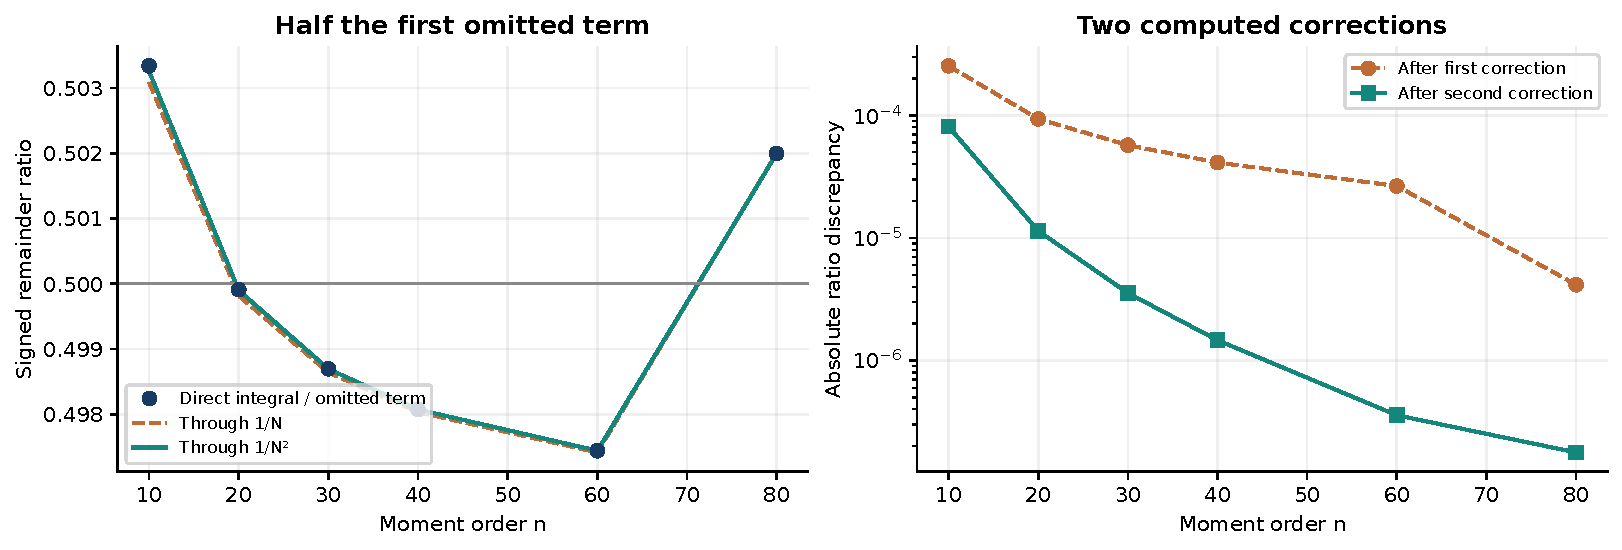
\includegraphics[width=\textwidth]{figures/moment_remainders.pdf}
 \caption{The signed error divided by the first omitted term, at a
 truncation near \((n+3/2)/\Lambda\). The first-correction formula tracks
 the small changes caused by rounding the truncation index. The plot is
 numerical corroboration; Theorem~\ref{thm:optimal-moment} supplies the proof.}
 \label{fig:moments}
\end{figure}

\subsection{A convergent identity with an explicit tail bound}

An asymptotic series should not be used as an infinite exact sum.
The same inverse coordinate gives an exact convergent alternative.

\begin{proposition}[Cutoff identity]\label{prop:cutoff}
For \(n\geq1\) and \(Y>\Lambda\),
\begin{equation}\label{eq:cutoff}
 m_n=\frac1{(n-1)!}\int_0^Y y^{n-1}g(e^{-y})\dd y
      +\sum_{k\geq1}\frac{c_k}{k^n}Q(n,kY),
 \qquad
 Q(n,z)=e^{-z}\sum_{j=0}^{n-1}\frac{z^j}{j!}.
\end{equation}
The sum is absolutely convergent. If \(Y>\log4\), the absolute tail
after \(k=K\) is at most
\begin{equation}\label{eq:cutoff-bound}
 \frac{(4e^{-Y})^{K+1}}{2(1-4e^{-Y})}
 \sum_{j=0}^{n-1}\frac{Y^j}{j!(K+1)^{n-j}}.
\end{equation}
\end{proposition}

\begin{proof}
Split \eqref{eq:layercake} at \(Y\), substitute the convergent inverse
series on the tail, and integrate term by term.
The coefficient growth theorem proves absolute convergence.
For the elementary explicit bound, note that
\[
 \frac{1/2}{\Phi(1/2)}=\frac1{2\sqrt\pi}>\frac14.
\]
The smaller solution to \(B=t\Phi(B)\) at \(t=1/4\) is therefore
less than \(1/2\); equivalently \(B(1/4)<1/2\).
Positivity gives \(b_k\leq4^k/2\).
For \(k>K\) and \(j\leq n-1\), \(k^{j-n}\leq(K+1)^{j-n}\).
The geometric tail now gives \eqref{eq:cutoff-bound}.
\end{proof}

The numerical implementation uses ordinary high-precision arithmetic
and explicitly distinguishes analytic truncation bounds from interval
rounding bounds. Formula \eqref{eq:cutoff} is also suitable for a future
ball-arithmetic evaluator: the finite inverse integral and all constant
evaluations can be enclosed separately.

